\documentclass[1p]{elsarticle_modified}
%\bibliographystyle{elsarticle-num}

%\usepackage[colorlinks]{hyperref}
%\usepackage{abbrmath_seonhwa} %\Abb, \Ascr, \Acal ,\Abf, \Afrak
\usepackage{amsfonts}
\usepackage{amssymb}
\usepackage{amsmath}
\usepackage{amsthm}
\usepackage{scalefnt}
\usepackage{amsbsy}
\usepackage{kotex}
\usepackage{caption}
\usepackage{subfig}
\usepackage{color}
\usepackage{graphicx}
\usepackage{xcolor} %% white, black, red, green, blue, cyan, magenta, yellow
\usepackage{float}
\usepackage{setspace}
\usepackage{hyperref}

\usepackage{tikz}
\usetikzlibrary{arrows}

\usepackage{multirow}
\usepackage{array} % fixed length table
\usepackage{hhline}

%%%%%%%%%%%%%%%%%%%%%
\makeatletter
\renewcommand*\env@matrix[1][\arraystretch]{%
	\edef\arraystretch{#1}%
	\hskip -\arraycolsep
	\let\@ifnextchar\new@ifnextchar
	\array{*\c@MaxMatrixCols c}}
\makeatother %https://tex.stackexchange.com/questions/14071/how-can-i-increase-the-line-spacing-in-a-matrix
%%%%%%%%%%%%%%%

\usepackage[normalem]{ulem}

\newcommand{\msout}[1]{\ifmmode\text{\sout{\ensuremath{#1}}}\else\sout{#1}\fi}
%SOURCE: \msout is \stkout macro in https://tex.stackexchange.com/questions/20609/strikeout-in-math-mode

\newcommand{\cancel}[1]{
	\ifmmode
	{\color{red}\msout{#1}}
	\else
	{\color{red}\sout{#1}}
	\fi
}

\newcommand{\add}[1]{
	{\color{blue}\uwave{#1}}
}

\newcommand{\replace}[2]{
	\ifmmode
	{\color{red}\msout{#1}}{\color{blue}\uwave{#2}}
	\else
	{\color{red}\sout{#1}}{\color{blue}\uwave{#2}}
	\fi
}

\newcommand{\Sol}{\mathcal{S}} %segment
\newcommand{\D}{D} %diagram
\newcommand{\A}{\mathcal{A}} %arc


%%%%%%%%%%%%%%%%%%%%%%%%%%%%%5 test

\def\sl{\operatorname{\textup{SL}}(2,\Cbb)}
\def\psl{\operatorname{\textup{PSL}}(2,\Cbb)}
\def\quan{\mkern 1mu \triangleright \mkern 1mu}

\theoremstyle{definition}
\newtheorem{thm}{Theorem}[section]
\newtheorem{prop}[thm]{Proposition}
\newtheorem{lem}[thm]{Lemma}
\newtheorem{ques}[thm]{Question}
\newtheorem{cor}[thm]{Corollary}
\newtheorem{defn}[thm]{Definition}
\newtheorem{exam}[thm]{Example}
\newtheorem{rmk}[thm]{Remark}
\newtheorem{alg}[thm]{Algorithm}

\newcommand{\I}{\sqrt{-1}}
\begin{document}

%\begin{frontmatter}
%
%\title{Boundary parabolic representations of knots up to 8 crossings}
%
%%% Group authors per affiliation:
%\author{Yunhi Cho} 
%\address{Department of Mathematics, University of Seoul, Seoul, Korea}
%\ead{yhcho@uos.ac.kr}
%
%
%\author{Seonhwa Kim} %\fnref{s_kim}}
%\address{Center for Geometry and Physics, Institute for Basic Science, Pohang, 37673, Korea}
%\ead{ryeona17@ibs.re.kr}
%
%\author{Hyuk Kim}
%\address{Department of Mathematical Sciences, Seoul National University, Seoul 08826, Korea}
%\ead{hyukkim@snu.ac.kr}
%
%\author{Seokbeom Yoon}
%\address{Department of Mathematical Sciences, Seoul National University, Seoul, 08826,  Korea}
%\ead{sbyoon15@snu.ac.kr}
%
%\begin{abstract}
%We find all boundary parabolic representation of knots up to 8 crossings.
%
%\end{abstract}
%\begin{keyword}
%    \MSC[2010] 57M25 
%\end{keyword}
%
%\end{frontmatter}

%\linenumbers
%\tableofcontents
%
\newcommand\colored[1]{\textcolor{white}{\rule[-0.35ex]{0.8em}{1.4ex}}\kern-0.8em\color{red} #1}%
%\newcommand\colored[1]{\textcolor{white}{ #1}\kern-2.17ex	\textcolor{white}{ #1}\kern-1.81ex	\textcolor{white}{ #1}\kern-2.15ex\color{red}#1	}

{\Large $\underline{12n_{0294}~(K12n_{0294})}$}

\setlength{\tabcolsep}{10pt}
\renewcommand{\arraystretch}{1.6}
\vspace{1cm}\begin{tabular}{m{100pt}>{\centering\arraybackslash}m{274pt}}
\multirow{5}{120pt}{
	\centering
	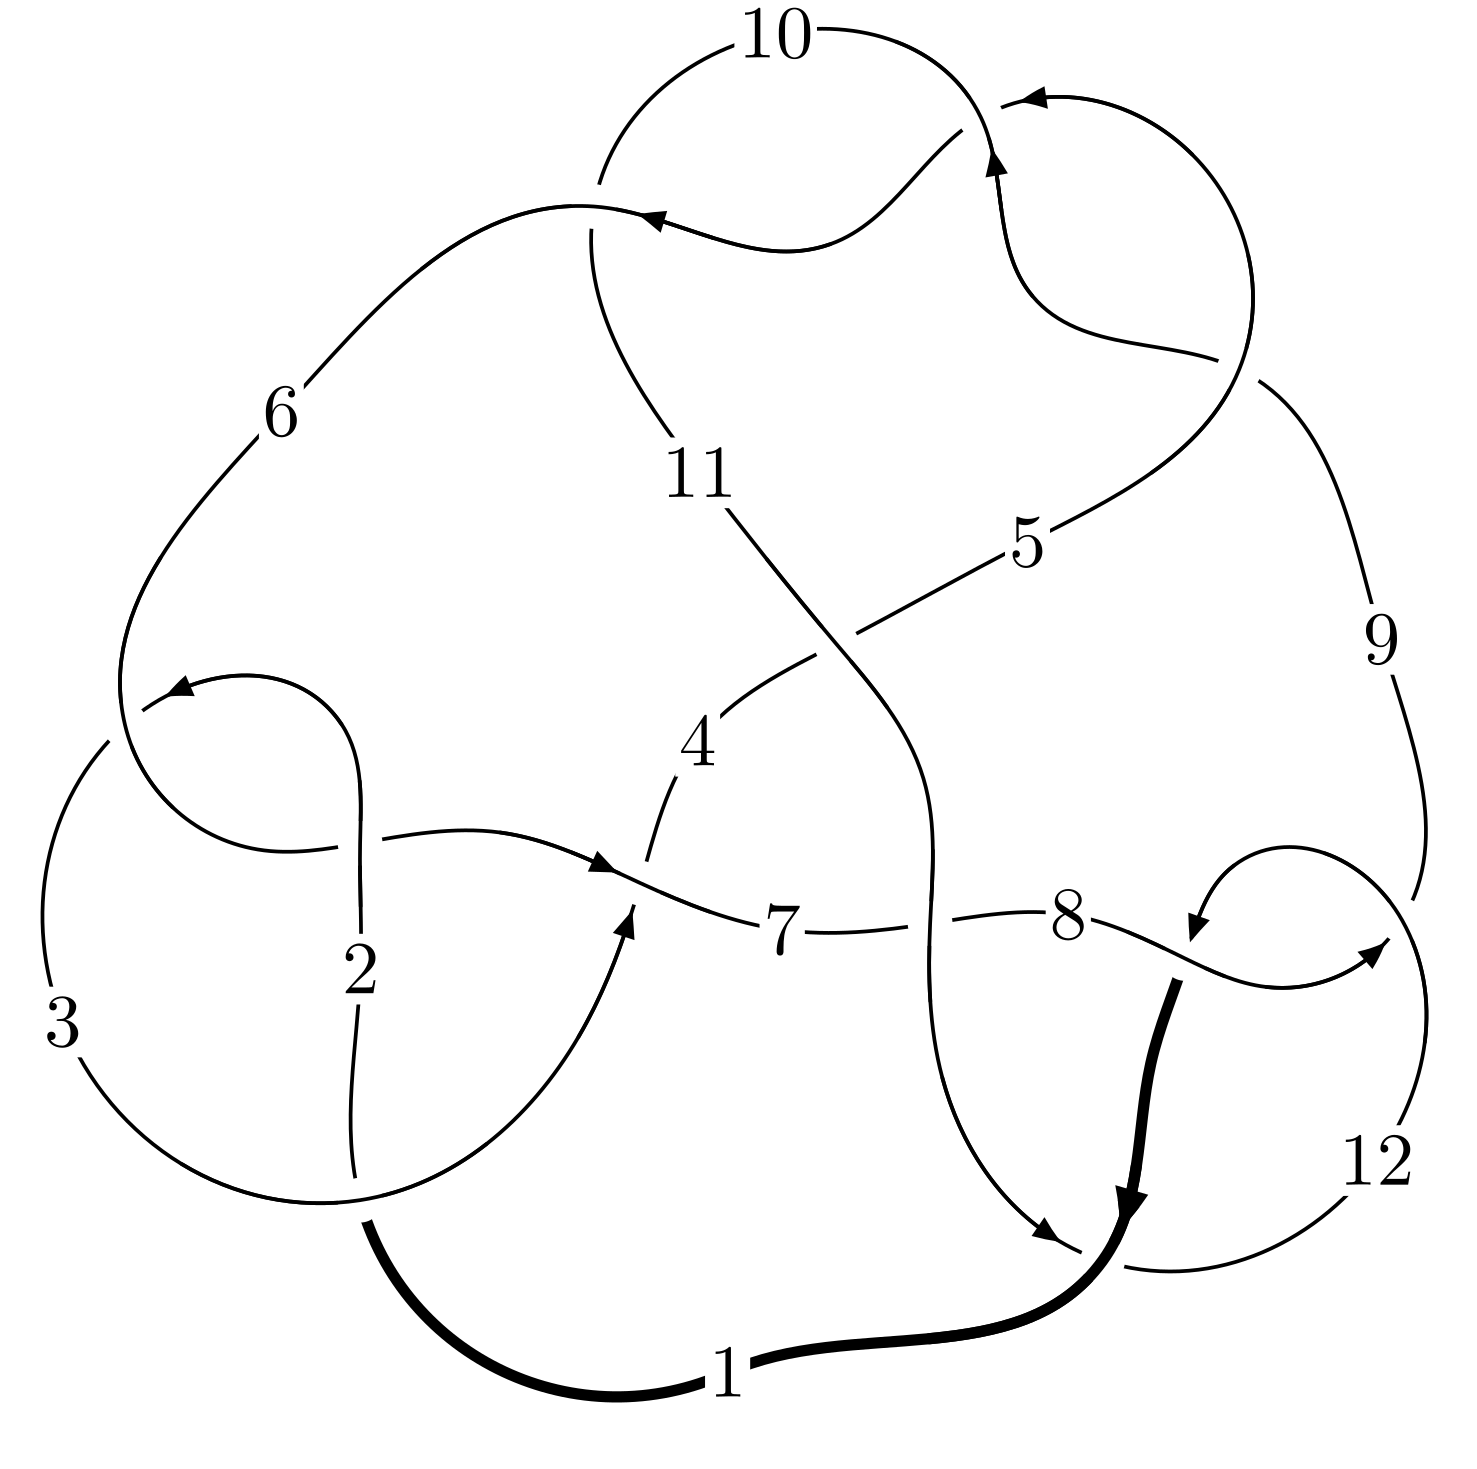
\includegraphics[width=112pt]{../../../GIT/diagram.site/Diagrams/png/2383_12n_0294.png}\\
\ \ \ A knot diagram\footnotemark}&
\allowdisplaybreaks
\textbf{Linearized knot diagam} \\
\cline{2-2}
 &
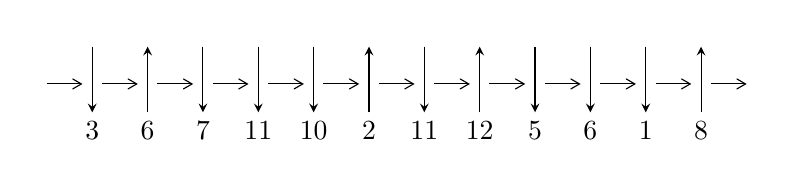
\begin{tikzpicture}[x=20pt, y=17pt]
	% nodes
	\node (C0) at (0, 0) {};
	\node (C1) at (1, 0) {};
	\node (C1U) at (1, +1) {};
	\node (C1D) at (1, -1) {3};

	\node (C2) at (2, 0) {};
	\node (C2U) at (2, +1) {};
	\node (C2D) at (2, -1) {6};

	\node (C3) at (3, 0) {};
	\node (C3U) at (3, +1) {};
	\node (C3D) at (3, -1) {7};

	\node (C4) at (4, 0) {};
	\node (C4U) at (4, +1) {};
	\node (C4D) at (4, -1) {11};

	\node (C5) at (5, 0) {};
	\node (C5U) at (5, +1) {};
	\node (C5D) at (5, -1) {10};

	\node (C6) at (6, 0) {};
	\node (C6U) at (6, +1) {};
	\node (C6D) at (6, -1) {2};

	\node (C7) at (7, 0) {};
	\node (C7U) at (7, +1) {};
	\node (C7D) at (7, -1) {11};

	\node (C8) at (8, 0) {};
	\node (C8U) at (8, +1) {};
	\node (C8D) at (8, -1) {12};

	\node (C9) at (9, 0) {};
	\node (C9U) at (9, +1) {};
	\node (C9D) at (9, -1) {5};

	\node (C10) at (10, 0) {};
	\node (C10U) at (10, +1) {};
	\node (C10D) at (10, -1) {6};

	\node (C11) at (11, 0) {};
	\node (C11U) at (11, +1) {};
	\node (C11D) at (11, -1) {1};

	\node (C12) at (12, 0) {};
	\node (C12U) at (12, +1) {};
	\node (C12D) at (12, -1) {8};
	\node (C13) at (13, 0) {};

	% arrows
	\draw[->,>={angle 60}]
	(C0) edge (C1) (C1) edge (C2) (C2) edge (C3) (C3) edge (C4) (C4) edge (C5) (C5) edge (C6) (C6) edge (C7) (C7) edge (C8) (C8) edge (C9) (C9) edge (C10) (C10) edge (C11) (C11) edge (C12) (C12) edge (C13) ;	\draw[->,>=stealth]
	(C1U) edge (C1D) (C2D) edge (C2U) (C3U) edge (C3D) (C4U) edge (C4D) (C5U) edge (C5D) (C6D) edge (C6U) (C7U) edge (C7D) (C8D) edge (C8U) (C9U) edge (C9D) (C10U) edge (C10D) (C11U) edge (C11D) (C12D) edge (C12U) ;
	\end{tikzpicture} \\
\hhline{~~} \\& 
\textbf{Solving Sequence} \\ \cline{2-2} 
 &
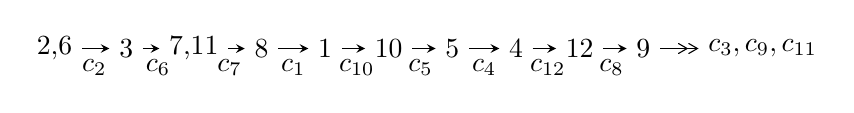
\begin{tikzpicture}[x=23pt, y=7pt]
	% node
	\node (A0) at (-1/8, 0) {2,6};
	\node (A1) at (1, 0) {3};
	\node (A2) at (33/16, 0) {7,11};
	\node (A3) at (25/8, 0) {8};
	\node (A4) at (33/8, 0) {1};
	\node (A5) at (41/8, 0) {10};
	\node (A6) at (49/8, 0) {5};
	\node (A7) at (57/8, 0) {4};
	\node (A8) at (65/8, 0) {12};
	\node (A9) at (73/8, 0) {9};
	\node (C1) at (1/2, -1) {$c_{2}$};
	\node (C2) at (3/2, -1) {$c_{6}$};
	\node (C3) at (21/8, -1) {$c_{7}$};
	\node (C4) at (29/8, -1) {$c_{1}$};
	\node (C5) at (37/8, -1) {$c_{10}$};
	\node (C6) at (45/8, -1) {$c_{5}$};
	\node (C7) at (53/8, -1) {$c_{4}$};
	\node (C8) at (61/8, -1) {$c_{12}$};
	\node (C9) at (69/8, -1) {$c_{8}$};
	\node (A10) at (11, 0) {$c_{3},c_{9},c_{11}$};

	% edge
	\draw[->,>=stealth]	
	(A0) edge (A1) (A1) edge (A2) (A2) edge (A3) (A3) edge (A4) (A4) edge (A5) (A5) edge (A6) (A6) edge (A7) (A7) edge (A8) (A8) edge (A9) ;
	\draw[->>,>={angle 60}]	
	(A9) edge (A10);
\end{tikzpicture} \\ 

\end{tabular} \\

\footnotetext{
The image of knot diagram is generated by the software ``\textbf{Draw programme}" developed by Andrew Bartholomew(\url{http://www.layer8.co.uk/maths/draw/index.htm\#Running-draw}), where we modified some parts for our purpose(\url{https://github.com/CATsTAILs/LinksPainter}).
}\phantom \\ \newline 
\centering \textbf{Ideals for irreducible components\footnotemark of $X_{\text{par}}$} 
 
\begin{align*}
I^u_{1}&=\langle 
u^{10}+u^9+5 u^8+4 u^7+9 u^6+6 u^5+3 u^4+3 u^3-5 u^2+2 b-1,\\
\phantom{I^u_{1}}&\phantom{= \langle  }u^{10}+u^9+5 u^8+4 u^7+9 u^6+6 u^5+3 u^4+3 u^3-7 u^2+2 a-3,\\
\phantom{I^u_{1}}&\phantom{= \langle  }u^{12}+u^{11}+5 u^{10}+4 u^9+10 u^8+7 u^7+7 u^6+6 u^5-2 u^4+3 u^3-3 u^2-1\rangle \\
I^u_{2}&=\langle 
-78963686 u^{21}-109276521 u^{20}+\cdots+272347738 b+755541991,\\
\phantom{I^u_{2}}&\phantom{= \langle  }207732146 u^{21}+642690277 u^{20}+\cdots+1906434166 a+152323303,\;u^{22}+2 u^{21}+\cdots+u+7\rangle \\
I^u_{3}&=\langle 
b- a- u,\;a^2+2 u,\;u^2- u+1\rangle \\
I^u_{4}&=\langle 
b+u,\;a,\;u^2+u+1\rangle \\
I^u_{5}&=\langle 
b- a+1,\;a^2+2 u,\;u^2- u+1\rangle \\
I^u_{6}&=\langle 
b+1,\;a,\;u^2+u+1\rangle \\
\\
\end{align*}
\raggedright * 6 irreducible components of $\dim_{\mathbb{C}}=0$, with total 46 representations.\\
\footnotetext{All coefficients of polynomials are rational numbers. But the coefficients are sometimes approximated in decimal forms when there is not enough margin.}
\newpage
\renewcommand{\arraystretch}{1}
\centering \section*{I. $I^u_{1}= \langle u^{10}+u^9+\cdots+2 b-1,\;u^{10}+u^9+\cdots+2 a-3,\;u^{12}+u^{11}+\cdots-3 u^2-1 \rangle$}
\flushleft \textbf{(i) Arc colorings}\\
\begin{tabular}{m{7pt} m{180pt} m{7pt} m{180pt} }
\flushright $a_{2}=$&$\begin{pmatrix}1\\0\end{pmatrix}$ \\
\flushright $a_{6}=$&$\begin{pmatrix}0\\u\end{pmatrix}$ \\
\flushright $a_{3}=$&$\begin{pmatrix}1\\- u^2\end{pmatrix}$ \\
\flushright $a_{7}=$&$\begin{pmatrix}u\\u\end{pmatrix}$ \\
\flushright $a_{11}=$&$\begin{pmatrix}-\frac{1}{2} u^{10}-\frac{1}{2} u^9+\cdots+\frac{7}{2} u^2+\frac{3}{2}\\-\frac{1}{2} u^{10}-\frac{1}{2} u^9+\cdots+\frac{5}{2} u^2+\frac{1}{2}\end{pmatrix}$ \\
\flushright $a_{8}=$&$\begin{pmatrix}\frac{1}{2} u^{11}+\frac{1}{2} u^{10}+\cdots- u^5-\frac{7}{2} u^3\\\frac{1}{2} u^{11}+\frac{1}{2} u^{10}+\cdots-\frac{3}{2} u^3+u\end{pmatrix}$ \\
\flushright $a_{1}=$&$\begin{pmatrix}u^2+1\\- u^4\end{pmatrix}$ \\
\flushright $a_{10}=$&$\begin{pmatrix}-\frac{1}{2} u^{10}-\frac{1}{2} u^9+\cdots+\frac{7}{2} u^2+\frac{3}{2}\\-\frac{1}{2} u^{10}-\frac{1}{2} u^9+\cdots+\frac{5}{2} u^2+1\end{pmatrix}$ \\
\flushright $a_{5}=$&$\begin{pmatrix}\frac{1}{2} u^{10}+u^9+\cdots-\frac{1}{2} u-\frac{1}{2}\\\frac{1}{2} u^{10}+u^9+\cdots-\frac{1}{2} u-1\end{pmatrix}$ \\
\flushright $a_{4}=$&$\begin{pmatrix}u^4+u^2+1\\u^4\end{pmatrix}$ \\
\flushright $a_{12}=$&$\begin{pmatrix}-\frac{1}{2} u^{10}-\frac{1}{2} u^9+\cdots+\frac{5}{2} u^2+\frac{3}{2}\\-\frac{1}{2} u^{10}-\frac{1}{2} u^9+\cdots+\frac{5}{2} u^2+\frac{1}{2}\end{pmatrix}$ \\
\flushright $a_{9}=$&$\begin{pmatrix}-\frac{1}{2} u^9-\frac{1}{2} u^8+\cdots- u^3+\frac{3}{2} u\\-\frac{1}{2} u^9-\frac{1}{2} u^8+\cdots+u^3+\frac{3}{2} u\end{pmatrix}$\\&\end{tabular}
\flushleft \textbf{(ii) Obstruction class $= -1$}\\~\\
\flushleft \textbf{(iii) Cusp Shapes $= -5 u^{11}-3 u^{10}-21 u^9-9 u^8-34 u^7-12 u^6-8 u^5-10 u^4+26 u^3-12 u^2+13 u-9$}\\~\\
\newpage\renewcommand{\arraystretch}{1}
\flushleft \textbf{(iv) u-Polynomials at the component}\newline \\
\begin{tabular}{m{50pt}|m{274pt}}
Crossings & \hspace{64pt}u-Polynomials at each crossing \\
\hline $$\begin{aligned}c_{1},c_{11}\end{aligned}$$&$\begin{aligned}
&u^{12}+9 u^{11}+\cdots+6 u+1
\end{aligned}$\\
\hline $$\begin{aligned}c_{2},c_{6},c_{8}\\c_{12}\end{aligned}$$&$\begin{aligned}
&u^{12}- u^{11}+5 u^{10}-4 u^9+10 u^8-7 u^7+7 u^6-6 u^5-2 u^4-3 u^3-3 u^2-1
\end{aligned}$\\
\hline $$\begin{aligned}c_{3},c_{7}\end{aligned}$$&$\begin{aligned}
&u^{12}+u^{11}+\cdots- u-2
\end{aligned}$\\
\hline $$\begin{aligned}c_{4}\end{aligned}$$&$\begin{aligned}
&u^{12}+15 u^{11}+\cdots+596 u+32
\end{aligned}$\\
\hline $$\begin{aligned}c_{5},c_{9},c_{10}\end{aligned}$$&$\begin{aligned}
&u^{12}-5 u^{11}+\cdots-4 u-4
\end{aligned}$\\
\hline
\end{tabular}\\~\\
\newpage\renewcommand{\arraystretch}{1}
\flushleft \textbf{(v) Riley Polynomials at the component}\newline \\
\begin{tabular}{m{50pt}|m{274pt}}
Crossings & \hspace{64pt}Riley Polynomials at each crossing \\
\hline $$\begin{aligned}c_{1},c_{11}\end{aligned}$$&$\begin{aligned}
&y^{12}-7 y^{11}+\cdots-10 y+1
\end{aligned}$\\
\hline $$\begin{aligned}c_{2},c_{6},c_{8}\\c_{12}\end{aligned}$$&$\begin{aligned}
&y^{12}+9 y^{11}+\cdots+6 y+1
\end{aligned}$\\
\hline $$\begin{aligned}c_{3},c_{7}\end{aligned}$$&$\begin{aligned}
&y^{12}-23 y^{11}+\cdots+51 y+4
\end{aligned}$\\
\hline $$\begin{aligned}c_{4}\end{aligned}$$&$\begin{aligned}
&y^{12}-35 y^{11}+\cdots-202128 y+1024
\end{aligned}$\\
\hline $$\begin{aligned}c_{5},c_{9},c_{10}\end{aligned}$$&$\begin{aligned}
&y^{12}-15 y^{11}+\cdots+16 y+16
\end{aligned}$\\
\hline
\end{tabular}\\~\\
\newpage\flushleft \textbf{(vi) Complex Volumes and Cusp Shapes}
$$\begin{array}{c|c|c}  
\text{Solutions to }I^u_{1}& \I (\text{vol} + \sqrt{-1}CS) & \text{Cusp shape}\\
 \hline 
\begin{aligned}
u &= -1.07086\phantom{ +0.000000I} \\
a &= \phantom{-}1.66252\phantom{ +0.000000I} \\
b &= -0.484232\phantom{ +0.000000I}\end{aligned}
 & -12.1281\phantom{ +0.000000I} & -5.69090\phantom{ +0.000000I} \\ \hline\begin{aligned}
u &= \phantom{-}0.296087 + 0.741679 I \\
a &= -0.55750 + 1.66481 I \\
b &= -1.09508 + 1.22561 I\end{aligned}
 & -5.57527 + 2.63814 I & -11.42884 - 2.06673 I \\ \hline\begin{aligned}
u &= \phantom{-}0.296087 - 0.741679 I \\
a &= -0.55750 - 1.66481 I \\
b &= -1.09508 - 1.22561 I\end{aligned}
 & -5.57527 - 2.63814 I & -11.42884 + 2.06673 I \\ \hline\begin{aligned}
u &= -0.162478 + 1.257750 I \\
a &= -0.651223 + 0.357840 I \\
b &= -0.095679 + 0.766555 I\end{aligned}
 & -5.08721 - 2.66459 I & -10.23667 + 3.12657 I \\ \hline\begin{aligned}
u &= -0.162478 - 1.257750 I \\
a &= -0.651223 - 0.357840 I \\
b &= -0.095679 - 0.766555 I\end{aligned}
 & -5.08721 + 2.66459 I & -10.23667 - 3.12657 I \\ \hline\begin{aligned}
u &= \phantom{-}0.635067\phantom{ +0.000000I} \\
a &= \phantom{-}1.51509\phantom{ +0.000000I} \\
b &= \phantom{-}0.111783\phantom{ +0.000000I}\end{aligned}
 & -1.87851\phantom{ +0.000000I} & -4.23810\phantom{ +0.000000I} \\ \hline\begin{aligned}
u &= \phantom{-}0.416797 + 1.329220 I \\
a &= -0.199126 - 0.960314 I \\
b &= \phantom{-}0.39398 - 2.06834 I\end{aligned}
 & -9.65412 + 7.95397 I & -10.78779 - 5.64533 I \\ \hline\begin{aligned}
u &= \phantom{-}0.416797 - 1.329220 I \\
a &= -0.199126 + 0.960314 I \\
b &= \phantom{-}0.39398 + 2.06834 I\end{aligned}
 & -9.65412 - 7.95397 I & -10.78779 + 5.64533 I \\ \hline\begin{aligned}
u &= -0.206233 + 0.541920 I \\
a &= \phantom{-}0.438428 - 0.668694 I \\
b &= -0.310427 - 0.445170 I\end{aligned}
 & -0.276323 - 1.063990 I & -4.38658 + 6.25986 I \\ \hline\begin{aligned}
u &= -0.206233 - 0.541920 I \\
a &= \phantom{-}0.438428 + 0.668694 I \\
b &= -0.310427 + 0.445170 I\end{aligned}
 & -0.276323 + 1.063990 I & -4.38658 - 6.25986 I\\
 \hline 
 \end{array}$$\newpage$$\begin{array}{c|c|c}  
\text{Solutions to }I^u_{1}& \I (\text{vol} + \sqrt{-1}CS) & \text{Cusp shape}\\
 \hline 
\begin{aligned}
u &= -0.62627 + 1.34351 I \\
a &= \phantom{-}0.380614 + 1.171480 I \\
b &= \phantom{-}0.79343 + 2.85430 I\end{aligned}
 & \phantom{-}19.3715 - 11.9727 I & -10.19562 + 5.57211 I \\ \hline\begin{aligned}
u &= -0.62627 - 1.34351 I \\
a &= \phantom{-}0.380614 - 1.171480 I \\
b &= \phantom{-}0.79343 - 2.85430 I\end{aligned}
 & \phantom{-}19.3715 + 11.9727 I & -10.19562 - 5.57211 I\\
 \hline 
 \end{array}$$\newpage\newpage\renewcommand{\arraystretch}{1}
\centering \section*{II. $I^u_{2}= \langle -7.90\times10^{7} u^{21}-1.09\times10^{8} u^{20}+\cdots+2.72\times10^{8} b+7.56\times10^{8},\;2.08\times10^{8} u^{21}+6.43\times10^{8} u^{20}+\cdots+1.91\times10^{9} a+1.52\times10^{8},\;u^{22}+2 u^{21}+\cdots+u+7 \rangle$}
\flushleft \textbf{(i) Arc colorings}\\
\begin{tabular}{m{7pt} m{180pt} m{7pt} m{180pt} }
\flushright $a_{2}=$&$\begin{pmatrix}1\\0\end{pmatrix}$ \\
\flushright $a_{6}=$&$\begin{pmatrix}0\\u\end{pmatrix}$ \\
\flushright $a_{3}=$&$\begin{pmatrix}1\\- u^2\end{pmatrix}$ \\
\flushright $a_{7}=$&$\begin{pmatrix}u\\u\end{pmatrix}$ \\
\flushright $a_{11}=$&$\begin{pmatrix}-0.108964 u^{21}-0.337116 u^{20}+\cdots-2.45446 u-0.0798996\\0.289937 u^{21}+0.401239 u^{20}+\cdots-0.514832 u-2.77418\end{pmatrix}$ \\
\flushright $a_{8}=$&$\begin{pmatrix}0.0918453 u^{21}+0.174181 u^{20}+\cdots+0.699627 u-0.598884\\0.113601 u^{21}+0.0746372 u^{20}+\cdots+2.03280 u-0.388234\end{pmatrix}$ \\
\flushright $a_{1}=$&$\begin{pmatrix}u^2+1\\- u^4\end{pmatrix}$ \\
\flushright $a_{10}=$&$\begin{pmatrix}-0.108964 u^{21}-0.337116 u^{20}+\cdots-2.45446 u-0.0798996\\0.308189 u^{21}+0.280109 u^{20}+\cdots-1.39677 u-3.60850\end{pmatrix}$ \\
\flushright $a_{5}=$&$\begin{pmatrix}0.0436157 u^{21}+0.236816 u^{20}+\cdots+0.624511 u+1.17524\\0.202828 u^{21}+0.763930 u^{20}+\cdots+1.77903 u+1.62345\end{pmatrix}$ \\
\flushright $a_{4}=$&$\begin{pmatrix}u^4+u^2+1\\u^4\end{pmatrix}$ \\
\flushright $a_{12}=$&$\begin{pmatrix}0.0937967 u^{21}+0.208563 u^{20}+\cdots-0.352346 u+1.14461\\0.592510 u^{21}+1.09915 u^{20}+\cdots+0.751139 u-3.19574\end{pmatrix}$ \\
\flushright $a_{9}=$&$\begin{pmatrix}0.121487 u^{21}+0.427747 u^{20}+\cdots+2.44535 u+0.605555\\-0.158323 u^{21}+0.138552 u^{20}+\cdots+1.87374 u+4.80979\end{pmatrix}$\\&\end{tabular}
\flushleft \textbf{(ii) Obstruction class $= -1$}\\~\\
\flushleft \textbf{(iii) Cusp Shapes $= -\frac{89419702}{136173869} u^{21}-\frac{42120566}{136173869} u^{20}+\cdots+\frac{1416145048}{136173869} u+\frac{452453139}{136173869}$}\\~\\
\newpage\renewcommand{\arraystretch}{1}
\flushleft \textbf{(iv) u-Polynomials at the component}\newline \\
\begin{tabular}{m{50pt}|m{274pt}}
Crossings & \hspace{64pt}u-Polynomials at each crossing \\
\hline $$\begin{aligned}c_{1},c_{11}\end{aligned}$$&$\begin{aligned}
&u^{22}+14 u^{21}+\cdots+307 u+49
\end{aligned}$\\
\hline $$\begin{aligned}c_{2},c_{6},c_{8}\\c_{12}\end{aligned}$$&$\begin{aligned}
&u^{22}-2 u^{21}+\cdots- u+7
\end{aligned}$\\
\hline $$\begin{aligned}c_{3},c_{7}\end{aligned}$$&$\begin{aligned}
&u^{22}+2 u^{21}+\cdots-145 u+35
\end{aligned}$\\
\hline $$\begin{aligned}c_{4}\end{aligned}$$&$\begin{aligned}
&(u^{11}-6 u^{10}+\cdots-48 u+32)^{2}
\end{aligned}$\\
\hline $$\begin{aligned}c_{5},c_{9},c_{10}\end{aligned}$$&$\begin{aligned}
&(u^{11}+2 u^{10}-7 u^9-14 u^8+17 u^7+32 u^6-20 u^5-30 u^4+9 u^3+8 u^2-2)^{2}
\end{aligned}$\\
\hline
\end{tabular}\\~\\
\newpage\renewcommand{\arraystretch}{1}
\flushleft \textbf{(v) Riley Polynomials at the component}\newline \\
\begin{tabular}{m{50pt}|m{274pt}}
Crossings & \hspace{64pt}Riley Polynomials at each crossing \\
\hline $$\begin{aligned}c_{1},c_{11}\end{aligned}$$&$\begin{aligned}
&y^{22}-10 y^{21}+\cdots-14085 y+2401
\end{aligned}$\\
\hline $$\begin{aligned}c_{2},c_{6},c_{8}\\c_{12}\end{aligned}$$&$\begin{aligned}
&y^{22}+14 y^{21}+\cdots+307 y+49
\end{aligned}$\\
\hline $$\begin{aligned}c_{3},c_{7}\end{aligned}$$&$\begin{aligned}
&y^{22}-34 y^{21}+\cdots+17965 y+1225
\end{aligned}$\\
\hline $$\begin{aligned}c_{4}\end{aligned}$$&$\begin{aligned}
&(y^{11}-58 y^{10}+\cdots+12928 y-1024)^{2}
\end{aligned}$\\
\hline $$\begin{aligned}c_{5},c_{9},c_{10}\end{aligned}$$&$\begin{aligned}
&(y^{11}-18 y^{10}+\cdots+32 y-4)^{2}
\end{aligned}$\\
\hline
\end{tabular}\\~\\
\newpage\flushleft \textbf{(vi) Complex Volumes and Cusp Shapes}
$$\begin{array}{c|c|c}  
\text{Solutions to }I^u_{2}& \I (\text{vol} + \sqrt{-1}CS) & \text{Cusp shape}\\
 \hline 
\begin{aligned}
u &= \phantom{-}0.315297 + 0.937809 I \\
a &= -0.373766 + 0.436547 I \\
b &= \phantom{-}0.57981 + 1.45156 I\end{aligned}
 & -0.82409 + 3.69934 I & -10.27594 - 2.30433 I \\ \hline\begin{aligned}
u &= \phantom{-}0.315297 - 0.937809 I \\
a &= -0.373766 - 0.436547 I \\
b &= \phantom{-}0.57981 - 1.45156 I\end{aligned}
 & -0.82409 - 3.69934 I & -10.27594 + 2.30433 I \\ \hline\begin{aligned}
u &= -0.621678 + 0.900743 I \\
a &= \phantom{-}0.433725 + 0.285994 I \\
b &= \phantom{-}0.477184 - 0.282729 I\end{aligned}
 & -0.82409 - 3.69934 I & -10.27594 + 2.30433 I \\ \hline\begin{aligned}
u &= -0.621678 - 0.900743 I \\
a &= \phantom{-}0.433725 - 0.285994 I \\
b &= \phantom{-}0.477184 + 0.282729 I\end{aligned}
 & -0.82409 + 3.69934 I & -10.27594 - 2.30433 I \\ \hline\begin{aligned}
u &= -1.140860 + 0.146410 I \\
a &= -1.58475 - 0.10382 I \\
b &= \phantom{-}0.383248 + 0.166816 I\end{aligned}
 & -16.3894 + 5.6976 I & -8.38395 - 2.57135 I \\ \hline\begin{aligned}
u &= -1.140860 - 0.146410 I \\
a &= -1.58475 + 0.10382 I \\
b &= \phantom{-}0.383248 - 0.166816 I\end{aligned}
 & -16.3894 - 5.6976 I & -8.38395 + 2.57135 I \\ \hline\begin{aligned}
u &= -0.528041 + 0.663736 I \\
a &= \phantom{-}0.036886 - 0.596779 I \\
b &= -0.411020 - 0.383825 I\end{aligned}
 & -0.153907 - 1.029650 I & -5.69847 + 5.62903 I \\ \hline\begin{aligned}
u &= -0.528041 - 0.663736 I \\
a &= \phantom{-}0.036886 + 0.596779 I \\
b &= -0.411020 + 0.383825 I\end{aligned}
 & -0.153907 + 1.029650 I & -5.69847 - 5.62903 I \\ \hline\begin{aligned}
u &= \phantom{-}0.797910 + 0.128505 I \\
a &= -1.42715 + 0.64453 I \\
b &= -0.302057 + 0.565900 I\end{aligned}
 & -5.23581 + 3.47501 I & -8.51244 - 3.77183 I \\ \hline\begin{aligned}
u &= \phantom{-}0.797910 - 0.128505 I \\
a &= -1.42715 - 0.64453 I \\
b &= -0.302057 - 0.565900 I\end{aligned}
 & -5.23581 - 3.47501 I & -8.51244 + 3.77183 I\\
 \hline 
 \end{array}$$\newpage$$\begin{array}{c|c|c}  
\text{Solutions to }I^u_{2}& \I (\text{vol} + \sqrt{-1}CS) & \text{Cusp shape}\\
 \hline 
\begin{aligned}
u &= \phantom{-}0.026101 + 1.195750 I \\
a &= -0.193214 - 1.265770 I \\
b &= \phantom{-}0.79244 - 2.46937 I\end{aligned}
 & -7.69899 - 1.57384 I & -11.44703 + 1.61053 I \\ \hline\begin{aligned}
u &= \phantom{-}0.026101 - 1.195750 I \\
a &= -0.193214 + 1.265770 I \\
b &= \phantom{-}0.79244 + 2.46937 I\end{aligned}
 & -7.69899 + 1.57384 I & -11.44703 - 1.61053 I \\ \hline\begin{aligned}
u &= \phantom{-}0.306447 + 1.162800 I \\
a &= \phantom{-}0.007196 + 1.052430 I \\
b &= -0.56018 + 1.99198 I\end{aligned}
 & -5.23581 + 3.47501 I & -8.51244 - 3.77183 I \\ \hline\begin{aligned}
u &= \phantom{-}0.306447 - 1.162800 I \\
a &= \phantom{-}0.007196 - 1.052430 I \\
b &= -0.56018 - 1.99198 I\end{aligned}
 & -5.23581 - 3.47501 I & -8.51244 + 3.77183 I \\ \hline\begin{aligned}
u &= \phantom{-}0.174005 + 0.725075 I \\
a &= \phantom{-}0.560735 - 0.384864 I \\
b &= -0.654598 - 0.645346 I\end{aligned}
 & -0.153907 - 1.029650 I & -5.69847 + 5.62903 I \\ \hline\begin{aligned}
u &= \phantom{-}0.174005 - 0.725075 I \\
a &= \phantom{-}0.560735 + 0.384864 I \\
b &= -0.654598 + 0.645346 I\end{aligned}
 & -0.153907 + 1.029650 I & -5.69847 - 5.62903 I \\ \hline\begin{aligned}
u &= \phantom{-}0.648660 + 1.107420 I \\
a &= \phantom{-}0.771605 - 0.910213 I \\
b &= \phantom{-}0.461513 - 1.169360 I\end{aligned}
 & -7.69899 + 1.57384 I & -11.44703 - 1.61053 I \\ \hline\begin{aligned}
u &= \phantom{-}0.648660 - 1.107420 I \\
a &= \phantom{-}0.771605 + 0.910213 I \\
b &= \phantom{-}0.461513 + 1.169360 I\end{aligned}
 & -7.69899 - 1.57384 I & -11.44703 + 1.61053 I \\ \hline\begin{aligned}
u &= -0.53111 + 1.36431 I \\
a &= -0.379457 - 1.188610 I \\
b &= -0.55682 - 2.99037 I\end{aligned}
 & -16.3894 - 5.6976 I & -8.38395 + 2.57135 I \\ \hline\begin{aligned}
u &= -0.53111 - 1.36431 I \\
a &= -0.379457 + 1.188610 I \\
b &= -0.55682 + 2.99037 I\end{aligned}
 & -16.3894 + 5.6976 I & -8.38395 - 2.57135 I\\
 \hline 
 \end{array}$$\newpage$$\begin{array}{c|c|c}  
\text{Solutions to }I^u_{2}& \I (\text{vol} + \sqrt{-1}CS) & \text{Cusp shape}\\
 \hline 
\begin{aligned}
u &= -0.44674 + 1.47157 I \\
a &= \phantom{-}0.362471 + 1.193990 I \\
b &= \phantom{-}0.29049 + 2.82389 I\end{aligned}
 & \phantom{-}17.8360\phantom{ +0.000000I} & -11.36432 + 0. I\phantom{ +0.000000I} \\ \hline\begin{aligned}
u &= -0.44674 - 1.47157 I \\
a &= \phantom{-}0.362471 - 1.193990 I \\
b &= \phantom{-}0.29049 - 2.82389 I\end{aligned}
 & \phantom{-}17.8360\phantom{ +0.000000I} & -11.36432 + 0. I\phantom{ +0.000000I}\\
 \hline 
 \end{array}$$\newpage\newpage\renewcommand{\arraystretch}{1}
\centering \section*{III. $I^u_{3}= \langle b- a- u,\;a^2+2 u,\;u^2- u+1 \rangle$}
\flushleft \textbf{(i) Arc colorings}\\
\begin{tabular}{m{7pt} m{180pt} m{7pt} m{180pt} }
\flushright $a_{2}=$&$\begin{pmatrix}1\\0\end{pmatrix}$ \\
\flushright $a_{6}=$&$\begin{pmatrix}0\\u\end{pmatrix}$ \\
\flushright $a_{3}=$&$\begin{pmatrix}1\\- u+1\end{pmatrix}$ \\
\flushright $a_{7}=$&$\begin{pmatrix}u\\u\end{pmatrix}$ \\
\flushright $a_{11}=$&$\begin{pmatrix}a\\a+u\end{pmatrix}$ \\
\flushright $a_{8}=$&$\begin{pmatrix}a u- a+u\\a u- a+u-1\end{pmatrix}$ \\
\flushright $a_{1}=$&$\begin{pmatrix}u\\u\end{pmatrix}$ \\
\flushright $a_{10}=$&$\begin{pmatrix}a\\- a u+2 a+u\end{pmatrix}$ \\
\flushright $a_{5}=$&$\begin{pmatrix}-2 u+2\\a u- a-3 u+2\end{pmatrix}$ \\
\flushright $a_{4}=$&$\begin{pmatrix}0\\- u\end{pmatrix}$ \\
\flushright $a_{12}=$&$\begin{pmatrix}a+1\\a+u+1\end{pmatrix}$ \\
\flushright $a_{9}=$&$\begin{pmatrix}- a\\- a- u\end{pmatrix}$\\&\end{tabular}
\flushleft \textbf{(ii) Obstruction class $= 1$}\\~\\
\flushleft \textbf{(iii) Cusp Shapes $= -8 u-4$}\\~\\
\newpage\renewcommand{\arraystretch}{1}
\flushleft \textbf{(iv) u-Polynomials at the component}\newline \\
\begin{tabular}{m{50pt}|m{274pt}}
Crossings & \hspace{64pt}u-Polynomials at each crossing \\
\hline $$\begin{aligned}c_{1},c_{2},c_{8}\\c_{11}\end{aligned}$$&$\begin{aligned}
&(u^2- u+1)^2
\end{aligned}$\\
\hline $$\begin{aligned}c_{3},c_{6},c_{7}\\c_{12}\end{aligned}$$&$\begin{aligned}
&(u^2+u+1)^2
\end{aligned}$\\
\hline $$\begin{aligned}c_{4},c_{5},c_{9}\\c_{10}\end{aligned}$$&$\begin{aligned}
&(u^2-2)^2
\end{aligned}$\\
\hline
\end{tabular}\\~\\
\newpage\renewcommand{\arraystretch}{1}
\flushleft \textbf{(v) Riley Polynomials at the component}\newline \\
\begin{tabular}{m{50pt}|m{274pt}}
Crossings & \hspace{64pt}Riley Polynomials at each crossing \\
\hline $$\begin{aligned}c_{1},c_{2},c_{3}\\c_{6},c_{7},c_{8}\\c_{11},c_{12}\end{aligned}$$&$\begin{aligned}
&(y^2+y+1)^2
\end{aligned}$\\
\hline $$\begin{aligned}c_{4},c_{5},c_{9}\\c_{10}\end{aligned}$$&$\begin{aligned}
&(y-2)^4
\end{aligned}$\\
\hline
\end{tabular}\\~\\
\newpage\flushleft \textbf{(vi) Complex Volumes and Cusp Shapes}
$$\begin{array}{c|c|c}  
\text{Solutions to }I^u_{3}& \I (\text{vol} + \sqrt{-1}CS) & \text{Cusp shape}\\
 \hline 
\begin{aligned}
u &= \phantom{-}0.500000 + 0.866025 I \\
a &= \phantom{-}0.707110 - 1.224740 I \\
b &= \phantom{-}1.207110 - 0.358719 I\end{aligned}
 & -4.93480 + 4.05977 I & -8.00000 - 6.92820 I \\ \hline\begin{aligned}
u &= \phantom{-}0.500000 + 0.866025 I \\
a &= -0.707110 + 1.224740 I \\
b &= -0.20711 + 2.09077 I\end{aligned}
 & -4.93480 + 4.05977 I & -8.00000 - 6.92820 I \\ \hline\begin{aligned}
u &= \phantom{-}0.500000 - 0.866025 I \\
a &= \phantom{-}0.707110 + 1.224740 I \\
b &= \phantom{-}1.207110 + 0.358719 I\end{aligned}
 & -4.93480 - 4.05977 I & -8.00000 + 6.92820 I \\ \hline\begin{aligned}
u &= \phantom{-}0.500000 - 0.866025 I \\
a &= -0.707110 - 1.224740 I \\
b &= -0.20711 - 2.09077 I\end{aligned}
 & -4.93480 - 4.05977 I & -8.00000 + 6.92820 I\\
 \hline 
 \end{array}$$\newpage\newpage\renewcommand{\arraystretch}{1}
\centering \section*{IV. $I^u_{4}= \langle b+u,\;a,\;u^2+u+1 \rangle$}
\flushleft \textbf{(i) Arc colorings}\\
\begin{tabular}{m{7pt} m{180pt} m{7pt} m{180pt} }
\flushright $a_{2}=$&$\begin{pmatrix}1\\0\end{pmatrix}$ \\
\flushright $a_{6}=$&$\begin{pmatrix}0\\u\end{pmatrix}$ \\
\flushright $a_{3}=$&$\begin{pmatrix}1\\u+1\end{pmatrix}$ \\
\flushright $a_{7}=$&$\begin{pmatrix}u\\u\end{pmatrix}$ \\
\flushright $a_{11}=$&$\begin{pmatrix}0\\- u\end{pmatrix}$ \\
\flushright $a_{8}=$&$\begin{pmatrix}u\\u+1\end{pmatrix}$ \\
\flushright $a_{1}=$&$\begin{pmatrix}- u\\- u\end{pmatrix}$ \\
\flushright $a_{10}=$&$\begin{pmatrix}0\\- u\end{pmatrix}$ \\
\flushright $a_{5}=$&$\begin{pmatrix}0\\u\end{pmatrix}$ \\
\flushright $a_{4}=$&$\begin{pmatrix}0\\u\end{pmatrix}$ \\
\flushright $a_{12}=$&$\begin{pmatrix}1\\- u+1\end{pmatrix}$ \\
\flushright $a_{9}=$&$\begin{pmatrix}0\\- u\end{pmatrix}$\\&\end{tabular}
\flushleft \textbf{(ii) Obstruction class $= 1$}\\~\\
\flushleft \textbf{(iii) Cusp Shapes $= 8 u+4$}\\~\\
\newpage\renewcommand{\arraystretch}{1}
\flushleft \textbf{(iv) u-Polynomials at the component}\newline \\
\begin{tabular}{m{50pt}|m{274pt}}
Crossings & \hspace{64pt}u-Polynomials at each crossing \\
\hline $$\begin{aligned}c_{1},c_{3},c_{6}\\c_{7},c_{11},c_{12}\end{aligned}$$&$\begin{aligned}
&u^2- u+1
\end{aligned}$\\
\hline $$\begin{aligned}c_{2},c_{8}\end{aligned}$$&$\begin{aligned}
&u^2+u+1
\end{aligned}$\\
\hline $$\begin{aligned}c_{4},c_{5},c_{9}\\c_{10}\end{aligned}$$&$\begin{aligned}
&u^2
\end{aligned}$\\
\hline
\end{tabular}\\~\\
\newpage\renewcommand{\arraystretch}{1}
\flushleft \textbf{(v) Riley Polynomials at the component}\newline \\
\begin{tabular}{m{50pt}|m{274pt}}
Crossings & \hspace{64pt}Riley Polynomials at each crossing \\
\hline $$\begin{aligned}c_{1},c_{2},c_{3}\\c_{6},c_{7},c_{8}\\c_{11},c_{12}\end{aligned}$$&$\begin{aligned}
&y^2+y+1
\end{aligned}$\\
\hline $$\begin{aligned}c_{4},c_{5},c_{9}\\c_{10}\end{aligned}$$&$\begin{aligned}
&y^2
\end{aligned}$\\
\hline
\end{tabular}\\~\\
\newpage\flushleft \textbf{(vi) Complex Volumes and Cusp Shapes}
$$\begin{array}{c|c|c}  
\text{Solutions to }I^u_{4}& \I (\text{vol} + \sqrt{-1}CS) & \text{Cusp shape}\\
 \hline 
\begin{aligned}
u &= -0.500000 + 0.866025 I \\
a &= \phantom{-0.000000 } 0 \\
b &= \phantom{-}0.500000 - 0.866025 I\end{aligned}
 & \phantom{-0.000000 } -4.05977 I & \phantom{-0.000000 -}0. + 6.92820 I \\ \hline\begin{aligned}
u &= -0.500000 - 0.866025 I \\
a &= \phantom{-0.000000 } 0 \\
b &= \phantom{-}0.500000 + 0.866025 I\end{aligned}
 & \phantom{-0.000000 -}4.05977 I & \phantom{-0.000000 } 0. - 6.92820 I\\
 \hline 
 \end{array}$$\newpage\newpage\renewcommand{\arraystretch}{1}
\centering \section*{V. $I^u_{5}= \langle b- a+1,\;a^2+2 u,\;u^2- u+1 \rangle$}
\flushleft \textbf{(i) Arc colorings}\\
\begin{tabular}{m{7pt} m{180pt} m{7pt} m{180pt} }
\flushright $a_{2}=$&$\begin{pmatrix}1\\0\end{pmatrix}$ \\
\flushright $a_{6}=$&$\begin{pmatrix}0\\u\end{pmatrix}$ \\
\flushright $a_{3}=$&$\begin{pmatrix}1\\- u+1\end{pmatrix}$ \\
\flushright $a_{7}=$&$\begin{pmatrix}u\\u\end{pmatrix}$ \\
\flushright $a_{11}=$&$\begin{pmatrix}a\\a-1\end{pmatrix}$ \\
\flushright $a_{8}=$&$\begin{pmatrix}- a u+u\\- a u+2 u\end{pmatrix}$ \\
\flushright $a_{1}=$&$\begin{pmatrix}u\\u\end{pmatrix}$ \\
\flushright $a_{10}=$&$\begin{pmatrix}a\\- a u+2 a-1\end{pmatrix}$ \\
\flushright $a_{5}=$&$\begin{pmatrix}-2 u+2\\- a u-3 u+2\end{pmatrix}$ \\
\flushright $a_{4}=$&$\begin{pmatrix}0\\- u\end{pmatrix}$ \\
\flushright $a_{12}=$&$\begin{pmatrix}a+u-1\\a+u-2\end{pmatrix}$ \\
\flushright $a_{9}=$&$\begin{pmatrix}- a\\- a+1\end{pmatrix}$\\&\end{tabular}
\flushleft \textbf{(ii) Obstruction class $= 1$}\\~\\
\flushleft \textbf{(iii) Cusp Shapes $= -8$}\\~\\
\newpage\renewcommand{\arraystretch}{1}
\flushleft \textbf{(iv) u-Polynomials at the component}\newline \\
\begin{tabular}{m{50pt}|m{274pt}}
Crossings & \hspace{64pt}u-Polynomials at each crossing \\
\hline $$\begin{aligned}c_{1},c_{2},c_{8}\\c_{11}\end{aligned}$$&$\begin{aligned}
&(u^2- u+1)^2
\end{aligned}$\\
\hline $$\begin{aligned}c_{3},c_{6},c_{7}\\c_{12}\end{aligned}$$&$\begin{aligned}
&(u^2+u+1)^2
\end{aligned}$\\
\hline $$\begin{aligned}c_{4},c_{5},c_{9}\\c_{10}\end{aligned}$$&$\begin{aligned}
&(u^2-2)^2
\end{aligned}$\\
\hline
\end{tabular}\\~\\
\newpage\renewcommand{\arraystretch}{1}
\flushleft \textbf{(v) Riley Polynomials at the component}\newline \\
\begin{tabular}{m{50pt}|m{274pt}}
Crossings & \hspace{64pt}Riley Polynomials at each crossing \\
\hline $$\begin{aligned}c_{1},c_{2},c_{3}\\c_{6},c_{7},c_{8}\\c_{11},c_{12}\end{aligned}$$&$\begin{aligned}
&(y^2+y+1)^2
\end{aligned}$\\
\hline $$\begin{aligned}c_{4},c_{5},c_{9}\\c_{10}\end{aligned}$$&$\begin{aligned}
&(y-2)^4
\end{aligned}$\\
\hline
\end{tabular}\\~\\
\newpage\flushleft \textbf{(vi) Complex Volumes and Cusp Shapes}
$$\begin{array}{c|c|c}  
\text{Solutions to }I^u_{5}& \I (\text{vol} + \sqrt{-1}CS) & \text{Cusp shape}\\
 \hline 
\begin{aligned}
u &= \phantom{-}0.500000 + 0.866025 I \\
a &= \phantom{-}0.707110 - 1.224740 I \\
b &= -0.292893 - 1.224750 I\end{aligned}
 & -4.93480\phantom{ +0.000000I} & -8.00000\phantom{ +0.000000I} \\ \hline\begin{aligned}
u &= \phantom{-}0.500000 + 0.866025 I \\
a &= -0.707110 + 1.224740 I \\
b &= -1.70711 + 1.22474 I\end{aligned}
 & -4.93480\phantom{ +0.000000I} & -8.00000\phantom{ +0.000000I} \\ \hline\begin{aligned}
u &= \phantom{-}0.500000 - 0.866025 I \\
a &= \phantom{-}0.707110 + 1.224740 I \\
b &= -0.292893 + 1.224750 I\end{aligned}
 & -4.93480\phantom{ +0.000000I} & -8.00000\phantom{ +0.000000I} \\ \hline\begin{aligned}
u &= \phantom{-}0.500000 - 0.866025 I \\
a &= -0.707110 - 1.224740 I \\
b &= -1.70711 - 1.22474 I\end{aligned}
 & -4.93480\phantom{ +0.000000I} & -8.00000\phantom{ +0.000000I}\\
 \hline 
 \end{array}$$\newpage\newpage\renewcommand{\arraystretch}{1}
\centering \section*{VI. $I^u_{6}= \langle b+1,\;a,\;u^2+u+1 \rangle$}
\flushleft \textbf{(i) Arc colorings}\\
\begin{tabular}{m{7pt} m{180pt} m{7pt} m{180pt} }
\flushright $a_{2}=$&$\begin{pmatrix}1\\0\end{pmatrix}$ \\
\flushright $a_{6}=$&$\begin{pmatrix}0\\u\end{pmatrix}$ \\
\flushright $a_{3}=$&$\begin{pmatrix}1\\u+1\end{pmatrix}$ \\
\flushright $a_{7}=$&$\begin{pmatrix}u\\u\end{pmatrix}$ \\
\flushright $a_{11}=$&$\begin{pmatrix}0\\-1\end{pmatrix}$ \\
\flushright $a_{8}=$&$\begin{pmatrix}u\\2 u\end{pmatrix}$ \\
\flushright $a_{1}=$&$\begin{pmatrix}- u\\- u\end{pmatrix}$ \\
\flushright $a_{10}=$&$\begin{pmatrix}0\\-1\end{pmatrix}$ \\
\flushright $a_{5}=$&$\begin{pmatrix}0\\u\end{pmatrix}$ \\
\flushright $a_{4}=$&$\begin{pmatrix}0\\u\end{pmatrix}$ \\
\flushright $a_{12}=$&$\begin{pmatrix}- u-1\\- u-2\end{pmatrix}$ \\
\flushright $a_{9}=$&$\begin{pmatrix}0\\-1\end{pmatrix}$\\&\end{tabular}
\flushleft \textbf{(ii) Obstruction class $= 1$}\\~\\
\flushleft \textbf{(iii) Cusp Shapes $= -6$}\\~\\
\newpage\renewcommand{\arraystretch}{1}
\flushleft \textbf{(iv) u-Polynomials at the component}\newline \\
\begin{tabular}{m{50pt}|m{274pt}}
Crossings & \hspace{64pt}u-Polynomials at each crossing \\
\hline $$\begin{aligned}c_{1},c_{3},c_{6}\\c_{7},c_{11},c_{12}\end{aligned}$$&$\begin{aligned}
&u^2- u+1
\end{aligned}$\\
\hline $$\begin{aligned}c_{2},c_{8}\end{aligned}$$&$\begin{aligned}
&u^2+u+1
\end{aligned}$\\
\hline $$\begin{aligned}c_{4},c_{5},c_{9}\\c_{10}\end{aligned}$$&$\begin{aligned}
&u^2
\end{aligned}$\\
\hline
\end{tabular}\\~\\
\newpage\renewcommand{\arraystretch}{1}
\flushleft \textbf{(v) Riley Polynomials at the component}\newline \\
\begin{tabular}{m{50pt}|m{274pt}}
Crossings & \hspace{64pt}Riley Polynomials at each crossing \\
\hline $$\begin{aligned}c_{1},c_{2},c_{3}\\c_{6},c_{7},c_{8}\\c_{11},c_{12}\end{aligned}$$&$\begin{aligned}
&y^2+y+1
\end{aligned}$\\
\hline $$\begin{aligned}c_{4},c_{5},c_{9}\\c_{10}\end{aligned}$$&$\begin{aligned}
&y^2
\end{aligned}$\\
\hline
\end{tabular}\\~\\
\newpage\flushleft \textbf{(vi) Complex Volumes and Cusp Shapes}
$$\begin{array}{c|c|c}  
\text{Solutions to }I^u_{6}& \I (\text{vol} + \sqrt{-1}CS) & \text{Cusp shape}\\
 \hline 
\begin{aligned}
u &= -0.500000 + 0.866025 I \\
a &= \phantom{-0.000000 } 0 \\
b &= -1.00000\phantom{ +0.000000I}\end{aligned}
 & \phantom{-0.000000 } 0 & -6.00000\phantom{ +0.000000I} \\ \hline\begin{aligned}
u &= -0.500000 - 0.866025 I \\
a &= \phantom{-0.000000 } 0 \\
b &= -1.00000\phantom{ +0.000000I}\end{aligned}
 & \phantom{-0.000000 } 0 & -6.00000\phantom{ +0.000000I}\\
 \hline 
 \end{array}$$\newpage
\newpage\renewcommand{\arraystretch}{1}
\centering \section*{ VII. u-Polynomials}
\begin{tabular}{m{50pt}|m{274pt}}
Crossings & \hspace{64pt}u-Polynomials at each crossing \\
\hline $$\begin{aligned}c_{1},c_{11}\end{aligned}$$&$\begin{aligned}
&((u^2- u+1)^6)(u^{12}+9 u^{11}+\cdots+6 u+1)\\
&\cdot(u^{22}+14 u^{21}+\cdots+307 u+49)
\end{aligned}$\\
\hline $$\begin{aligned}c_{2},c_{8}\end{aligned}$$&$\begin{aligned}
&(u^2- u+1)^4(u^2+u+1)^2\\
&\cdot(u^{12}- u^{11}+5 u^{10}-4 u^9+10 u^8-7 u^7+7 u^6-6 u^5-2 u^4-3 u^3-3 u^2-1)\\
&\cdot(u^{22}-2 u^{21}+\cdots- u+7)
\end{aligned}$\\
\hline $$\begin{aligned}c_{3},c_{7}\end{aligned}$$&$\begin{aligned}
&((u^2- u+1)^2)(u^2+u+1)^4(u^{12}+u^{11}+\cdots- u-2)\\
&\cdot(u^{22}+2 u^{21}+\cdots-145 u+35)
\end{aligned}$\\
\hline $$\begin{aligned}c_{4}\end{aligned}$$&$\begin{aligned}
&u^4(u^2-2)^4(u^{11}-6 u^{10}+\cdots-48 u+32)^{2}\\
&\cdot(u^{12}+15 u^{11}+\cdots+596 u+32)
\end{aligned}$\\
\hline $$\begin{aligned}c_{5},c_{9},c_{10}\end{aligned}$$&$\begin{aligned}
&u^4(u^2-2)^4\\
&\cdot(u^{11}+2 u^{10}-7 u^9-14 u^8+17 u^7+32 u^6-20 u^5-30 u^4+9 u^3+8 u^2-2)^{2}\\
&\cdot(u^{12}-5 u^{11}+\cdots-4 u-4)
\end{aligned}$\\
\hline $$\begin{aligned}c_{6},c_{12}\end{aligned}$$&$\begin{aligned}
&(u^2- u+1)^2(u^2+u+1)^4\\
&\cdot(u^{12}- u^{11}+5 u^{10}-4 u^9+10 u^8-7 u^7+7 u^6-6 u^5-2 u^4-3 u^3-3 u^2-1)\\
&\cdot(u^{22}-2 u^{21}+\cdots- u+7)
\end{aligned}$\\
\hline
\end{tabular}\newpage\renewcommand{\arraystretch}{1}
\centering \section*{ VIII. Riley Polynomials}
\begin{tabular}{m{50pt}|m{274pt}}
Crossings & \hspace{64pt}Riley Polynomials at each crossing \\
\hline $$\begin{aligned}c_{1},c_{11}\end{aligned}$$&$\begin{aligned}
&((y^2+y+1)^6)(y^{12}-7 y^{11}+\cdots-10 y+1)\\
&\cdot(y^{22}-10 y^{21}+\cdots-14085 y+2401)
\end{aligned}$\\
\hline $$\begin{aligned}c_{2},c_{6},c_{8}\\c_{12}\end{aligned}$$&$\begin{aligned}
&((y^2+y+1)^6)(y^{12}+9 y^{11}+\cdots+6 y+1)\\
&\cdot(y^{22}+14 y^{21}+\cdots+307 y+49)
\end{aligned}$\\
\hline $$\begin{aligned}c_{3},c_{7}\end{aligned}$$&$\begin{aligned}
&((y^2+y+1)^6)(y^{12}-23 y^{11}+\cdots+51 y+4)\\
&\cdot(y^{22}-34 y^{21}+\cdots+17965 y+1225)
\end{aligned}$\\
\hline $$\begin{aligned}c_{4}\end{aligned}$$&$\begin{aligned}
&y^4(y-2)^8(y^{11}-58 y^{10}+\cdots+12928 y-1024)^{2}\\
&\cdot(y^{12}-35 y^{11}+\cdots-202128 y+1024)
\end{aligned}$\\
\hline $$\begin{aligned}c_{5},c_{9},c_{10}\end{aligned}$$&$\begin{aligned}
&y^4(y-2)^8(y^{11}-18 y^{10}+\cdots+32 y-4)^{2}\\
&\cdot(y^{12}-15 y^{11}+\cdots+16 y+16)
\end{aligned}$\\
\hline
\end{tabular}
\vskip 2pc
\end{document}